\makeatletter
\def\input@path{{../styles/}{../../styles/}{../../../styles/}{../}{../../}{../../../}}
\makeatother
\documentclass{ee102_notes}
% macros.tex - Course meta information
\renewcommand{\course}{EE 102}
\renewcommand{\coursetitle}{Signal Processing and Linear Systems}
\renewcommand{\instructor}{Ayush Pandey}
\renewcommand{\semester}{Fall}
\renewcommand{\year}{2025}
\renewcommand{\shorttitle}{Week 1: Introduction to Signals}
% Use \renewcommand to avoid 'already defined' errors

% The following packages can be found on http:\\www.ctan.org
% \usepackage{graphics} % for pdf, bitmapped graphics files
%\usepackage{epsfig} % for postscript graphics files
%\usepackage{mathptmx} % assumes new font selection scheme installed
%\usepackage{times} % assumes new font selection scheme installed
\usepackage{amsmath} % assumes amsmath package installed
\usepackage{amssymb,mathtools}  % assumes amsmath package installed
\usepackage{xcolor}
\usepackage{pgfplots,subcaption}
\usepackage[hidelinks]{hyperref}
\usepackage{verbatim}
\usepackage{graphicx}
\usepackage{listings}
\usepackage{fancyhdr}
% \usepackage{geometry}
\usepackage{siunitx}
\usepackage[most]{tcolorbox}
\usepackage{enumitem}
\usepackage{environ}
% -------- listings (Python) ----------
\lstdefinestyle{py}{
  language=Python,
  basicstyle=\ttfamily\small,
  keywordstyle=\color{blue!60!black}\bfseries,
  commentstyle=\color{green!40!black},
  stringstyle=\color{orange!60!black},
  showstringspaces=false,
  columns=fullflexible,
  frame=single,
  framerule=0.3pt,
  numbers=left,
  numberstyle=\tiny,
  xleftmargin=1em,
  tabsize=2,
  breaklines=true,
}

\usepackage[american]{circuitikz}
\usepackage{tikz}
\usetikzlibrary{arrows.meta,positioning,calc,angles,quotes}
\tikzset{
  >={Latex[length=2.2mm]},
  block/.style={draw, thick, rectangle, minimum height=10mm, minimum width=24mm, align=center},
  gain/.style={block, minimum width=14mm},
  sum/.style={draw, thick, circle, inner sep=0pt, minimum size=6mm},
  conn/.style={-Latex, thick},
}
\usepackage{caption}    
\usepackage{lscape}
\usepackage{soul}
\usepackage{physics}
\usepackage{hyperref}
\hypersetup{
    colorlinks=true,
    linkcolor=blue,
    filecolor=magenta,      
    urlcolor=blue,
    pdftitle={week1_notes},
    pdfpagemode=FullScreen,
}
%\usepackage{float} 

%\usepackage[demo]{graphicx}
\pgfplotsset{compat=1.18}
% \usepgfplotslibrary{fillbetween}

\newsavebox{\measurebox}

\let\proof\relax\let\endproof\relax


\def\abs#1{\left\lvert#1\right\rvert}
\let\proof\relax
\let\endproof\relax
\usepackage{amsthm}
\usepackage{accents}
\usepackage{relsize}
\newcommand{\ubar}[1]{\underaccent{\bar}{#1}}
\newtheorem{theorem}{Theorem}
\newtheorem{corollary}{Corollary}[theorem]
\newtheorem{lemma}{Lemma}
\newtheorem{proposition}{Proposition}
\newtheorem{statement}{Statement}

\theoremstyle{definition}
\newtheorem{definition}{Definition}
 
\theoremstyle{remark}
\newtheorem*{remark}{Remark}
\theoremstyle{remark}
\newtheorem*{claim}{Claim}
\setlength{\parindent}{0cm}
\newenvironment{nalign}{
    \begin{equation}
    \begin{aligned}
}{
    \end{aligned}
    \end{equation}
    \ignorespacesafterend
}

\renewcommand{\releasedate}{September 22, 2025}

\newcommand{\Eblank}{\rule{3cm}{0.4pt}}
\newcommand{\Rankblank}{\rule{3cm}{0.4pt}}

\begin{document}

\section*{EE 102 Week 4, Lecture 1 (Fall 2025)}
\subsection*{Instructor: \instructor}
\subsection*{Date: \releasedate}

\section{Goals for today}
To understand how to compute the output of a linear-time invariant system given any general input signal that is applied to the system. 
\section{Representing signals using impulses}
We have discussed the three fundamental signals: the unit step, the unit impulse, and the complex exponential. What's common about all three of these functions? Why are these three signals so special? The answer is that these three signals can be used to represent any arbitrary signal (well, almost any!) --- especially the signals that we come across in engineering practice. In the previous lectures, we have discussed how to write general signals only by using unit steps and complex exponentials. We have also briefly discussed how the definition of the unit impulse (in the sense of distributions), is in fact, a definition that says that each signal is made up of its samples at each time point and the impulse is the function that does the sampling. Let's try to break this down further with some examples. 

\subsection{Discrete-time step using impulse}
To help you build intuition for this concept, consider a signal in discrete-time. For example, the unit step signal $u[n]$ is defined as
\[
u[n] = \begin{cases}
1, & n \geq 0 \\
0, & n < 0
\end{cases}
\]
which can be visualized as a train of unit impulses as shown in Figure \ref{fig:d-t-unit-step}. It is clear that it is a signal that is made up of many impulses (see pop quiz below).

\begin{popquiz}
In discrete-time, write the unit step signal $u[n]$ as a sum of scaled and shifted unit impulses $\delta[n]$. 
\popqsplit
Notice that for any given value of $n$, the unit step $u[n]$ is equal to 1 if $n \geq 0$ and 0 otherwise. This means that the unit step can be viewed as a sum of all the unit impulses $\delta[k]$ for $k$ from $-\infty$ to $n$. So, we can write
\[
u[n] = \sum_{k=-\infty}^{n} \delta[k]
\]
for all $n \in \mathbb{Z}$. To represent the signal in terms of the general impulse $\delta[n]$, we can write:
\[
u[n] = \sum_{k=0}^{\infty} \delta[n-k].
\]
You can see that for any given $n$, the sum will only include the impulses from $k=0$ to $k=n$, which corresponds to the definition of the unit step. 
\end{popquiz}
\begin{figure}[h]
\centering
\begin{tikzpicture}[scale=1.0]
    % Draw axes
    \draw[->] (-5,0) -- (5,0) node[right] {$n$};
    \draw[->] (0,-1) -- (0,3) node[above] {$u[n]$};

    % Draw unit step
    \foreach \x in {0,1,2,3,4} {
        \draw[thick] (\x,0) -- (\x,2);
        \filldraw[black] (\x,2) circle (2pt);
    }
    \draw[thick] (-5,0) -- (0,0);
    \filldraw[black] (0,2) circle (2pt);

    % Add labels
    \node at (1,-0.5) {1};
    \node at (2,-0.5) {2};
    \node at (3,-0.5) {3};
    \node at (4,-0.5) {4};
    \node at (-1,-0.5) {-1};
    \node at (-2,-0.5) {-2};
    \node at (-3,-0.5) {-3};
    \node at (-4,-0.5) {-4};
    \node at (0.5,2.5) {};
\end{tikzpicture}

\caption{Unit step signal $u[n]$ visualized as a train of unit impulses.}
\label{fig:d-t-unit-step}
\end{figure} 


We see that the unit step can be viewed as many impulses (one impulse at each time point). This is also true for every other signal --- the simplest way to break down a signal is to view it as a sample at each time point. The unit impulse helps us pick out the samples at each time point so that we can write the logic above formally. A visualization of this idea is shown in Figure~\ref{fig:dt-impulse-sum}. 

\begin{figure}[h]
\centering

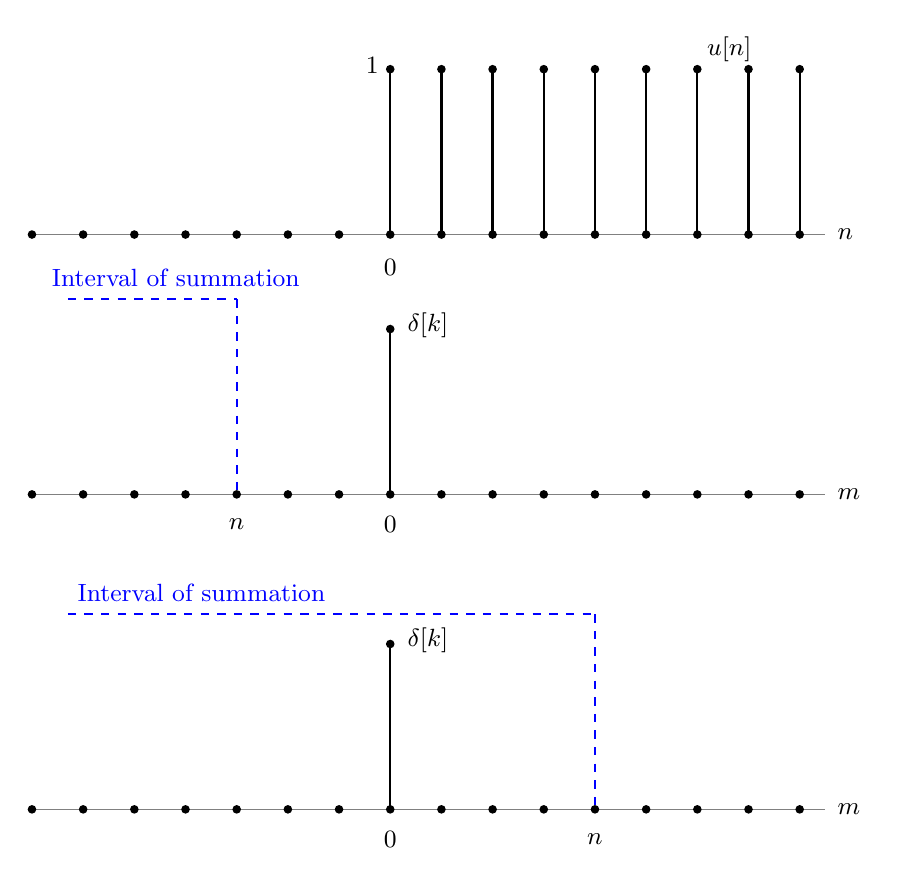
\begin{tikzpicture}[>=stealth, x=0.65cm, y=2.1cm]
  \tikzset{
    dot/.style={circle, fill=black, inner sep=1.1pt},
    stem/.style={thick},
    dashint/.style={blue, dashed, thick},
    axisline/.style={gray},
    txt/.style={font=\small}
  }

  \def\xmin{-7}  \def\xmax{8}
  \def\nmarkL{-3} % panel 2: n is to the LEFT of 0
  \def\nmarkR{4}  % panel 3: n is to the RIGHT of 0

  \begin{scope}[yshift=1.8cm]
    \draw[axisline] (\xmin,0) -- (\xmax+0.5,0);
    \foreach \k in {\xmin,...,\xmax} \node[dot] at (\k,0) {};
    % unit step u[n]
    \foreach \k in {0,...,\xmax} {
      \draw[stem] (\k,0) -- (\k,1);
      \node[dot] at (\k,1) {};
    }
    % labels
    \node[txt,anchor=west] at (\xmax+0.55,0) {$n$};
    \node[txt] at (-0.35,1.02) {$1$};
    \node[txt] at (0,-0.2) {$0$};
    \node[txt,anchor=west] at (6.0,1.12) {$u[n]$};
  \end{scope}


  \begin{scope}[yshift=-1.5cm]
    \draw[axisline] (\xmin,0) -- (\xmax+0.5,0);
    \foreach \k in {\xmin,...,\xmax} \node[dot] at (\k,0) {};
    % impulse δ[m]
    \draw[stem] (0,0) -- (0,1);
    \node[dot] at (0,1) {};
    \node[txt,anchor=west] at (0.15,1.02) {$\delta[k]$};
    \node[txt,anchor=west] at (\xmax+0.55,0) {$m$};
    % axis tick labels: n (left of 0) and 0
    \node[txt] at (\nmarkL,-0.18) {$n$};
    \node[txt] at (0,-0.18) {$0$};
    % blue dashed interval: from far left up to n (left of 0)
    \draw[dashint] (\xmin+0.7,1.18) -- (\nmarkL,1.18);
    \draw[dashint] (\nmarkL,1.18) -- (\nmarkL,0);
    \node[txt,anchor=west,blue] at (\xmin+0.2,1.31) {Interval of summation};
  \end{scope}
  \begin{scope}[yshift=-5.5cm]
    \draw[axisline] (\xmin,0) -- (\xmax+0.5,0);
    \foreach \k in {\xmin,...,\xmax} \node[dot] at (\k,0) {};
    % impulse δ[m]
    \draw[stem] (0,0) -- (0,1);
    \node[dot] at (0,1) {};
    \node[txt,anchor=west] at (0.15,1.02) {$\delta[k]$};
    \node[txt,anchor=west] at (\xmax+0.55,0) {$m$};
    % axis tick labels: 0 and n (right of 0)
    \node[txt] at (0,-0.18) {$0$};
    \node[txt] at (\nmarkR,-0.18) {$n$};
    % blue dashed interval: from far left up to n (right of 0)
    \draw[dashint] (\xmin+0.7,1.18) -- (\nmarkR,1.18);
    \draw[dashint] (\nmarkR,1.18) -- (\nmarkR,0);
    \node[txt,anchor=west,blue] at (\xmin+0.7,1.31) {Interval of summation};
  \end{scope}
\end{tikzpicture}

\caption{Visualization of the running sum representation of the unit step signal $u[n]$ as a sum of shifted impulses.}
\label{fig:dt-impulse-sum}
\end{figure}

\subsection{Impulse as a sampler in continuous-time}
Recall the sampling property of the impulse in continuous-time:
\[
\int_{-\infty}^{\infty} x(t) \delta(t - t_0) dt = x(t_0).
\]
This property tells us that the impulse function $\delta(t - t_0)$ acts as a sampler that picks out the value of the signal $x(t)$ at the specific time $t = t_0$. This means that we can represent any continuous-time signal $x(t)$ as an integral of scaled and shifted impulses. 
\subsection{Example: Representing a sinusoidal signal using impulses}
Let's work through this with a specific example of a sinusoidal signal: $x(t) = \sin(t)$. We can write $\sin(0)$ as
\[
\sin(0) = \int_{-\infty}^{\infty} \sin(\tau) \delta(\tau - 0) d\tau.
\]
Similarly, we can write $\sin(t_1)$ for any arbitrary time $t_1$ as
\[
\sin(t_1) = \int_{-\infty}^{\infty} \sin(\tau) \delta(\tau - t_1) d\tau.
\]
This means that we can represent the entire signal $\sin(t)$ as an integral of scaled and shifted impulses:
\[
\sin(t) = \int_{-\infty}^{\infty} \sin(\tau) \delta(\tau - t) d\tau.
\]
Now, this might seem trivial or even circular! But the key insight here is that we are expressing the signal as a continuous superposition of impulses, each weighted by the value of the signal at that point in time. 

\subsection{General representation of signals using impulses}
In general, any continuous-time signal $x(t)$ can be represented using impulses. Let's visualize an arbitrary signal $x(t)$ and see how it can be decomposed into impulses at each time point (see Figure~\ref{fig:ct-impulse-samplers}).
\begin{figure}[h]
\centering
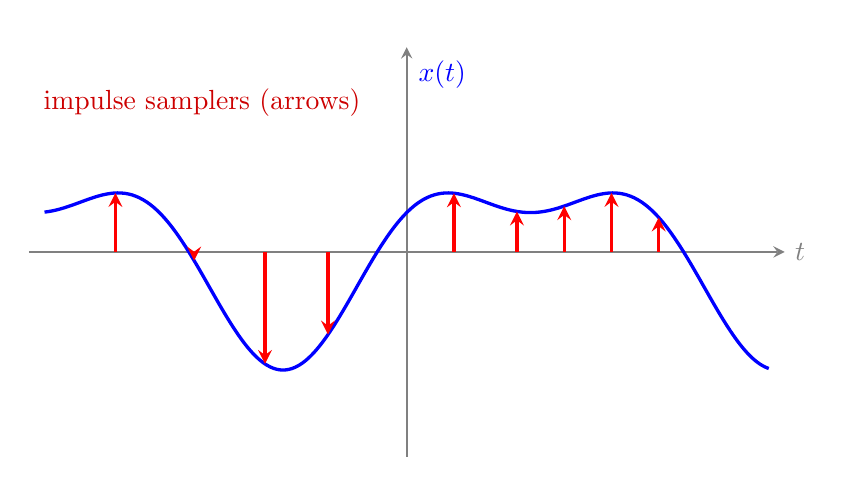
\begin{tikzpicture}[x=1cm,y=1cm,>=stealth]
  % --- axes ---
  \draw[->,gray,thick] (-4.8,0) -- (4.8,0) node[right] {$t$};
  \draw[->,gray,thick] (0,-2.6) -- (0,2.6) node[above] {};

  % --- signal x(t) ---
  \draw[very thick,blue,domain=-4.6:4.6,samples=200,smooth,variable=\t]
        plot ({\t},{sin(\t r) + 0.5*cos(2*\t r)});
  \node[blue] at (0.45,2.25) {$x(t)$};
  \node[red!80!black] at (-2.6,1.9) {impulse samplers (arrows)};

  % --- sampling instants ---
  \def\samples{-3.7,-2.7,-1.8,-1.0,0.6,1.4,2.0,2.6,3.2}

  % --- arrows that start on the x-axis and point to the curve ---
  \foreach \tt in \samples{
    \pgfmathsetmacro{\yy}{sin(\tt r) + 0.5*cos(2*\tt r)}
    % arrow from (t,0) to (t, y(t)), head at the curve
    \draw[red,very thick,-stealth] (\tt,0) -- (\tt,\yy);
  }
\end{tikzpicture}
\caption{Impulse samplers drawn as arrows from the time axis to the signal $x(t)$ (arrowheads at the curve).}
\label{fig:ct-impulse-samplers}
\end{figure}


At each point, the impulse signal can be written by shifting the impulse to that point and scaling it by the value of the signal at that point. Therefore, we start with $\delta(t)$ as the impulse at $t=0$. To get the impulse at an arbitrary time $t=\tau$, we shift the impulse to that point, which gives us $\delta(t - \tau)$. To scale this impulse by the value of the signal at that point, we multiply it by $x(\tau)$, resulting in $x(\tau) \delta(t - \tau)$. So, we have
\[
x(t) = \int_{-\infty}^{\infty} x(\tau) \delta(t - \tau) d\tau.
\]
\section{General output of an LTI system using impulse response}
We finally get to the main goal of this lecture. Our goal is to compute the output of systems given any arbitrary input signal. This is very important because in practice, we often encounter signals that are not as simple as the unit step or the complex exponential. We need a systematic way to compute the output of a system for any input signal. Think about the following examples, where we might want to compute the output of a system:
\begin{itemize}
    \item An audio signal (your recorded voice singing a song, for example) that needs to be filtered to remove noise. How would you represent your filtered signal mathematically (to be able to analyze and report back its properties to your music producer!)?
    \item For an integrated circuit, you might want to compute the output voltage of a circuit given an arbitrary input voltage signal (in real-world, the voltage signal is never a perfect sinusoid!).
    \item In communications, you might want to compute the output of a communication channel given an arbitrary input signal (for example, a modulated signal carrying information).
\end{itemize}
To achieve all of the above, we start by describing the impulse response of the system.

\subsection{Impulse response of an LTI system}
We define the impulse response of a system as the output of the system when the input is an impulse signal. In continuous-time, if the system input is $\delta(t)$, then we call the output of this system, the impulse response and denote it as $h(t)$ (see Figure~\ref{fig:impulse-response}).
\begin{figure}[h]
\centering
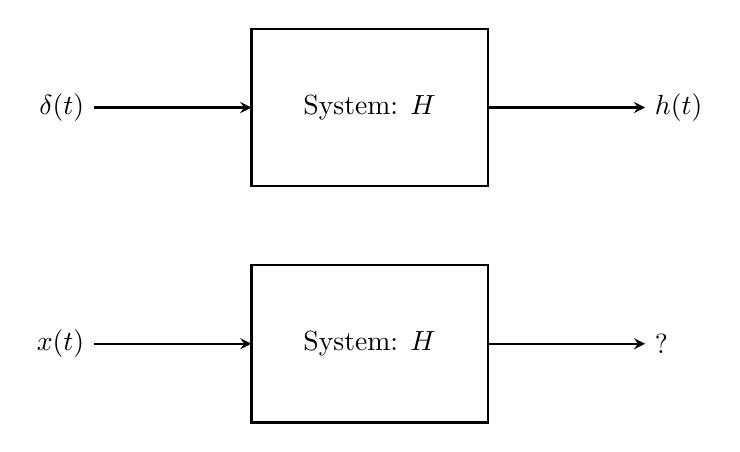
\begin{tikzpicture}[>=stealth, x=1cm, y=1
cm]
  % Draw the system box
  \draw[thick] (0,0) rectangle (3,2);
  \node at (1.5,1) {System: $H$};

  % Input arrow and label
  \draw[->, thick] (-2,1) -- (0,1);
  \node[anchor=east] at (-2,1) {$\delta(t)$};

  % Output arrow and label
  \draw[->, thick] (3,1) -- (5,1);
  \node[anchor=west] at (5,1) {$h(t)$};

  % add another box with x(t) input and ? output
    \draw[thick] (0,-3) rectangle (3,-1);
    \node at (1.5,-2) {System: $H$};
    % Input arrow and label
    \draw[->, thick] (-2,-2) -- (0,-2);
    \node[anchor=east] at (-2,-2) {$x(t)$};
    % Output arrow and label
    \draw[->, thick] (3,-2) -- (5,-2);
    \node[anchor=west] at (5,-2) {$?$};

    % Labels
    % \node at (1.5,2.3) {Impulse Response};
\end{tikzpicture}
\caption{Impulse response of a system: output $h(t)$ when input is $\delta(t)$. What is the output for a general input $x(t)$?}
\label{fig:impulse-response}
\end{figure}
Now, the question is, what is the output of the system when the input is an arbitrary signal $x(t)$? 
\begin{popquiz}
    What is the output of the system for a shifted impulse input $\delta(t - \tau)$? Do you need additional assumptions about the system to answer this question?
    \popqsplit
    To answer this question, we need to assume that the system is time-invariant. This means that if the input is shifted in time, the output will also be shifted by the same amount. Therefore, if the input is $\delta(t - \tau)$, the output will be $h(t - \tau)$.
\end{popquiz}

\begin{popquiz}
    What is the output of the system for a scaled impulse $k \delta(t)$? Do you need additional assumptions about the system to answer this question?
    \popqsplit
    To answer this question, we need to assume that the system is linear. This means that if the input is scaled by a constant factor, the output will also be scaled by the same factor. Therefore, if the input is $k \delta(t)$, the output will be $k h(t)$.
\end{popquiz}
We start by writing the output of the system for a shifted and scaled impulse input. That is, if the input is $x(\tau) \delta(t - \tau)$, then the output will be $x(\tau) h(t - \tau)$ (only if, of course, the system is linear and time-invariant!).
Now, we can write the output of the system for an arbitrary input $x(t)$ (see Figure~\ref{fig:convolution-buildup}) by using the integral representation of the input signal using impulses:
\begin{figure}[h]
\centering
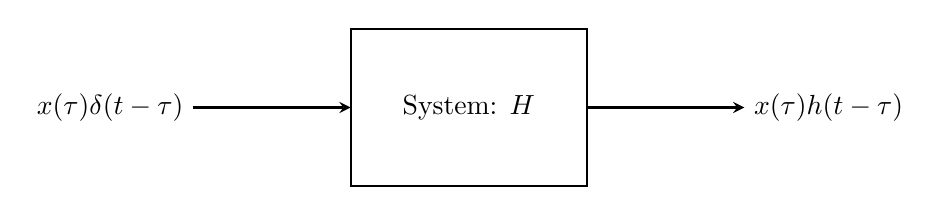
\begin{tikzpicture}[>=stealth, x=1cm, y=1
cm]
  % Draw the system box
  \draw[thick] (0,0) rectangle (3,2);
  \node at (1.5,1) {System: $H$};

  % Input arrow and label
  \draw[->, thick] (-2,1) -- (0,1);
  \node[anchor=east] at (-2,1) {$x(\tau)\delta(t - \tau)$};

  % Output arrow and label
  \draw[->, thick] (3,1) -- (5,1);
  \node[anchor=west] at (5,1) {$x(\tau)h(t - \tau)$};
\end{tikzpicture}
\caption{Impulse response of a system: output $h(t)$ when input is $\delta(t)$. What is the output for a general input $x(t)$?}
\label{fig:convolution-buildup}
\end{figure}
So, using the integral representation of the input signal, we can write the output of the system as
\[
y(t) = \int_{-\infty}^{\infty} x(\tau) h(t - \tau) d\tau.
\]
This integral is called the convolution integral, and it is denoted by the symbol $*$. Therefore, we can write the output of the system as
\[
y(t) = x(t) * h(t).
\]
\begin{popquiz}
    Write the discrete-time version of the convolution integral.
    \popqsplit
    In discrete-time, the convolution integral becomes a sum. Therefore, we can write the output of the system as
    \[
    y[n] = \sum_{k=-\infty}^{\infty} x[k] h[n - k].
    \]
    This sum is called the convolution sum, and it is also denoted by the symbol $*$.
\end{popquiz}
\section{Virtual manipulatives to understand convolution}
In the next lecture, we will use virtual manipulatives to understand convolution better. We will also discuss some properties of convolution and how to compute convolution using graphical methods (with many practical examples!).
\end{document}